\section{Récepteurs étudiés et acquisition}\label{sec:recepteurs-etudies-et-acquisition}
   Notre étude est orientée autour de deux récepteurs GNSS de coût et capacités différentes, l'un étant supposé être plus précis que l'autre.
   Nous allons donc chercher à prendre des mesures à l'aide de ces deux récepteurs afin de les étudier et entre autres de vérifier cette supposition.

   \subsection{Premier récepteur}\label{subsec:premier-recepteur-:-gpstar}
      Le premier récepteur, qui est celui que nous avons le plus utilisé lors de la prise de mesures, est le G Star IV de la marque \textit{GlobalSat}.
      Il s'agit d'un récepteur uniquement GPS, de petite taille, ce qui en fait un outil portable relativement précis permettant aisément d'effectuer des relevés de position grâce à un ordinateur.

      \begin{figure}[h]
          \centering
          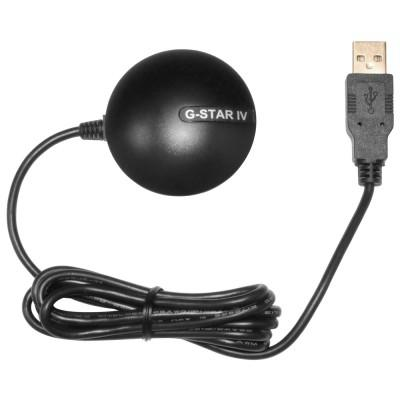
\includegraphics[width=.4\textwidth]{imgs/gstar}
          \caption{Récepteur G Star IV}
          \label{fig:gstar}
      \end{figure}

      Une fois branché en USB à un ordinateur, il est possible d'exploiter ses prises de mesures.
      Le récepteur transmettant les données reçues depuis les satellites émetteurs sous forme de suite de bits qu'il est possible de lire grâce au module \texttt{Serial} de Python, il est cependant nécessaire d'effectuer une traduction afin de rendre les données exploitables.

      En effet, les données sont donc transmises \textit{via} USB comme une suite de bits.
      Il faut donc tout d'abord organiser ces bits en octets, puis convertir chaque octet en valeur associée à un caractère de texte encodé selon la norme UTF-8.

      Une fois les données converties, il est intéressant de remarquer qu'elles suivent le format NMEA\@.
      Nous les enregistrons donc dans un fichier texte qu'il sera possible d'exploiter ultérieurement.

   \subsection{Second récepteur}\label{subsec:second-recepteur}
      Le second récepteur étudié est le SP80 de \textit{Spectra Geospatial}.
      Contrairement au premier récepteur, il est bien plus précis mais surtout bien plus imposant.
      Il possède, de plus, la capacité de recevoir des données aussi bien depuis le système GPS que depuis les systèmes GLONASS et Beidou.

      \begin{figure}[h]
          \centering
          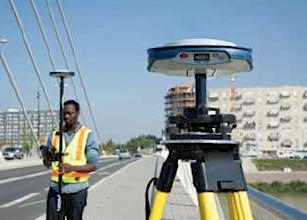
\includegraphics[width=.45\textwidth]{imgs/sp80}
          \caption{Récepteur SP80}
          \label{fig:sp80}
      \end{figure}

      Il se place alors naturellement comme un récepteur GNSS à usage d'avantage professionnel, pour des opérations nécessitant une précision conséquente.

      Concernant l'acquisition, le procédé est similaire, la transmission par USB s'effectuant de la même manière.